\section{JonDonym nutzen}
\textbf{JonDo} ist das Client-Programm f�r JonDonym, welches jeder Nutzer des Anonymisierungsdienstes JonDonym auf seinem Rechner installieren muss. Das Programm dient als Proxy f�r verschiedene Internet Applikationen. Der Datenverkehr wird verschl�sselt und an eine Mix-Kaskade weitergeleitet. Ein GUI erm�glicht die Konfiguration.\\

JonDo ist in Java implementiert und damit unter verschiedenen Betriebssystem nutzbar. Es gibt auch eine Version ohne GUI: JonDoConsole.
\begin{enumerate}
\item F�r \textbf{WINDOWS} ist als erstes ein Java Runtime Environment zu installieren. Den Installer f�r die aktuelle Version kann man von \textit{www.java.com} herunter laden. Bei der Installation m�chte der Installer unbedingt die \textit{Ask-Toolbar} f�r alle Browser installieren. Diese Option sollte man deaktivieren (Bild \ref{abb:asktoolbar}), braucht man nicht.\\

\begin{figure}[htb]
\begin{center}
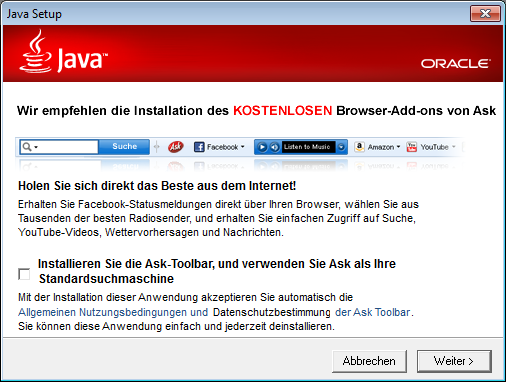
\includegraphics[scale=0.55]{../screenshots/java-install.png}
\caption{Installation der Ask-Toolbar deaktivieren}
\label{abb:asktoolbar}
\end{center}
\end{figure}

WICHTIG: Der Installer aktiviert auch ein Java-Plugin f�r alle Browser. Dieses Plug-in ist ein Sicherheitsrisiko und muss im Java Control Panel unter \textit{Systemsteuerung - Programme - Java} deaktiviert werden!
\begin{center}
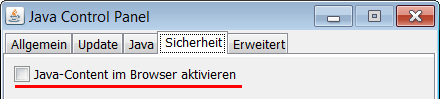
\includegraphics[scale=0.55]{../screenshots/java-ctrl-klein.png}
\end{center}

Die Downloadseite\footnote{ \href{https://www.anonym-surfen.de/jondo.html}{https://www.anonym-surfen.de/jondo.html}} von JonDonym bietet ein Setup Programm f�r JonDo. Es besteht die M�glichkeit, JonDo auf dem Rechner als Programm zu installieren, oder als portable Version auf dem USB-Stick. F�r die portable Installation auf dem USB-Stick braucht man keine Administratorrechte und es wird die ben�tigte Portable Java JRE installiert.\\

\begin{figure}[htb]
\begin{center}
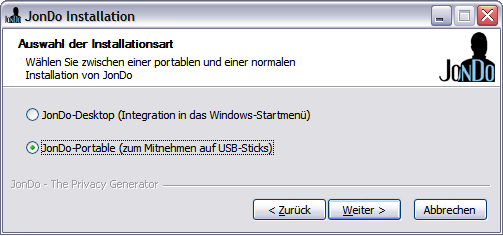
\includegraphics[scale=0.55]{../screenshots/jondo_inst1.png}
\caption{Installation von JonDo}
\label{abb:japinst}
\end{center}
\end{figure}

Im Anschluss an die portable Installation wird angeboten, auch gleich den JonDoFox (portable Version) f�r anonymes Surfen zu installieren.